%%%%%latex preamble%%%%%
\documentclass[titlepage]{article}\usepackage[]{graphicx}\usepackage[]{color}
%% maxwidth is the original width if it is less than linewidth
%% otherwise use linewidth (to make sure the graphics do not exceed the margin)
\makeatletter
\def\maxwidth{ %
  \ifdim\Gin@nat@width>\linewidth
  \linewidth
  \else
  \Gin@nat@width
  \fi
}
\makeatother


\usepackage{fancybox}


\usepackage{listings}
\definecolor{mygreen}{rgb}{0,0.6,0}
\definecolor{mygray}{rgb}{0.5,0.5,0.5}
\definecolor{mymauve}{rgb}{0.58,0,0.82}
\lstset{ %
  backgroundcolor=\color{white},   % choose the background color; you must add \usepackage{color} or \usepackage{xcolor}
  basicstyle=\footnotesize,        % the size of the fonts that are used for the code
  breakatwhitespace=false,         % sets if automatic breaks should only happen at whitespace
  breaklines=true,                 % sets automatic line breaking
  captionpos=b,                    % sets the caption-position to bottom
  commentstyle=\color{mygreen},    % comment style
  deletekeywords={...},            % if you want to delete keywords from the given language
  escapeinside={\%*}{*)},          % if you want to add LaTeX within your code
  extendedchars=true,              % lets you use non-ASCII characters; for 8-bits encodings only, does not work with UTF-8
  frame=single,                    % adds a frame around the code
  keepspaces=true,                 % keeps spaces in text, useful for keeping indentation of code (possibly needs columns=flexible)
  keywordstyle=\color{blue},       % keyword style
  language=Python,                 % the language of the code
  morekeywords={*,...},            % if you want to add more keywords to the set
  numbers=left,                    % where to put the line-numbers; possible values are (none, left, right)
  numbersep=5pt,                   % how far the line-numbers are from the code
  numberstyle=\tiny\color{mygray}, % the style that is used for the line-numbers
  rulecolor=\color{black},         % if not set, the frame-color may be changed on line-breaks within not-black text (e.g. comments (green here))
  showspaces=false,                % show spaces everywhere adding particular underscores; it overrides 'showstringspaces'
  showstringspaces=false,          % underline spaces within strings only
  showtabs=false,                  % show tabs within strings adding particular underscores
  stepnumber=2,                    % the step between two line-numbers. If it's 1, each line will be numbered
  stringstyle=\color{mymauve},     % string literal style
  tabsize=2,                       % sets default tabsize to 2 spaces
  title=\lstname                   % show the filename of files included with \lstinputlisting; also try caption instead of title
}
\usepackage{tikz}
\usetikzlibrary{external}
\usetikzlibrary{through}
\usetikzlibrary{plotmarks}
\usetikzlibrary{arrows,shapes}
\usetikzlibrary{plothandlers}
\usetikzlibrary{positioning}
\usetikzlibrary{calc}
\usepackage{alltt}
\usepackage[sc]{mathpazo}
\usepackage{amsmath, amsthm, amssymb}
\usepackage{graphicx}
\usepackage[T1]{fontenc}
\usepackage{geometry}
\geometry{verbose,tmargin=2.5cm,bmargin=2.5cm,lmargin=1.5cm,rmargin=1.5cm}
\setcounter{secnumdepth}{2}
\setcounter{tocdepth}{2}
\usepackage{url}
\usepackage[unicode=true,pdfusetitle,
  bookmarks=true,bookmarksnumbered=true,bookmarksopen=true,bookmarksopenlevel=2,
breaklinks=false,pdfborder={0 0 1},backref=false,colorlinks=false]
{hyperref}
\hypersetup{pdfstartview={XYZ null null 1}}
\usepackage{float}
\usepackage{bm}
\usepackage{tikz}
 %changes default sectioning commands -> 1,a, etc.
%\usepackage{breakurl}
\renewcommand{\thesubsection}{(\alph{subsection})}
\renewcommand{\thesubsubsection}{\roman{subsection}.}
\usepackage{lastpage}
\usepackage{fancyhdr}
\pagestyle{fancy}

%%% Header and Footer %%% 
\lhead{}
\chead{\leftmark}
\rhead{}
\lfoot{Aaron Gonzales; Algorithms}
\cfoot{Homework 2}
\rfoot{Page \thepage\ of \pageref{LastPage}}
\IfFileExists{upquote.sty}{\usepackage{upquote}}{}

\usetikzlibrary{arrows}



\begin{document}
\title{Homework 3 \\ dynamic programming, buying donuts, \\ and other such
things\\  CS561, \\ Fall 2014}
\author{Aaron Gonzales}
\maketitle


\section{Chip Testing }

\begin{quote}
\textbf{Professor Diogenes has $n$ supposedly identical integrated-circuit chips that
in principle are capable of testing each other. The professor's test jib
accommodates two chips at a time. When the jig is loaded, each chip tests the
other and reports whether it is good or bad. A good chip always reports
accurately whether the other chip is good or bad, but the professor cannot
trust the answer of a bad chip. Thus the following possible outcomes of a test
are as follows:}

\begin{table}[h]
\centering
  \begin{tabular}{lll}
	\hline
	\multicolumn{1}{|l|}{Chip A Says} & \multicolumn{1}{l|}{Chip B Says} & \multicolumn{1}{l|}{Conclusion} \\ \hline
	B is good                         & A is good                        & both are good, or both are bad  \\ \hline
	B is good                         & A is bad                         & at least one is bad             \\ \hline
	B is bad                          & A is good                        & at least one is bad             \\ \hline
	B is bad                          & A is bad                         & at least one is bad             \\ \hline
	\end{tabular}
  \end{table}

\end{quote}


\subsection{}
  \begin{quote}
\textbf{show that if more than $n/2$ chips are bad, the professor cannot
	necessarily determine which chips are good using any strategy based on this
	kind of pairwise test. Assume that the bad chips can conspire to fool the
	professor. }
  \end{quote}

\subsubsection{Answer}
The key assumption here is that the bad chips can conspire to fool the professor.
Here, let $B$ be the set of bad chips and $A$ be the set of good chips. As
$B>A$, there is a subset $b \subseteq B > A$ that can conspire to fool the
professor. Assuming they will try to do so, they will succeed, as they can
eventually weed out the good chips. 

  \subsection{ }
  \begin{quote}
  \textbf{consider the problem of finding a single good chip from among $n$ chips,
	assuming that more than $n/2$ of the chips are good. Show that $\lfloor n/2 \rfloor$ 
	pairwise tests are sufficient to reduce the problem to one of nearly
	half the size.}
  \end{quote}

  \subsubsection{Answer}
  If we call a single chip $c$ from the set of chips $C=\{c_1,\dots c_n\}$ and
  pair the chips to test them (e.g., $(c_i, c_{i+1})$ for $i = 1 \text{ to } n/2$

  each test of pairs can have two outcomes that we care about: 
  \begin{align*}
	  test (c_i, c_j) = \begin{cases}
		  A: \text{ at least one chip is reported bad} \\
		  B: \text{ both chips are reported good} 
	  \end{cases}
  \end{align*}

  for all tests with outcome A, we throw out both of the chips. Otherwise, we
  keep the pairs of chips with outcome B for further testing (we can call that
  set of pairs of potentially good chips $G$. From there, we remove one of the
  chips in each pair until we have one good chip left. We can then use that
  chip to test any other chip, since we know it's good. 

  
  \subsection{}
  \begin{quote}
  \textbf{show that the good chips can be identified with $\Theta(n)$ pairwise tests,
	assuming that more than $n/2$ chips are good. Give and solve the recurrence
	that describes the number of tests. }
  \end{quote}
  \subsubsection{answer}
  since we do $n/2$ pairwise comparisons and recursively remove chips from
  pairs, we get a relation of $ T(n) = (\frac{n}{2}) + \frac{n}{2} $. 
  The master method shows us that this becomes $\Theta(n)$. 






\section{Parenthesization }
\textbf{
  \begin{quote}
	Show via induction that a full Parenthesization of an $n$ element expression
	has exactly $n-1$ pairs of parenthesis. 
  \end{quote}
}

We start by saying the function $P(n)$ is the function that gives the number of
pairs of parentheses for $n$ matrices. 
Proof by induction:
\begin{proof}
\begin{align*}
  \text{if } P(j) =& j -1 \forall j < n \\
  \text{Base case: } P(1) =& 1-1 = 0 \text{ (no parentheses for 1 matrix)}\\
  \text{Inductive Hypothesis: } P(n) =& P(n-1) \forall n \geq 2 \\
  \text{Inductive Step: } \forall n \geq 2, P(n) =& P(n-1)+1 \text{ (by IH)}\\
  P(n-1) =& (n-1-1) = n - 2 \\
  P(n-1)+1 =& n -2 +1 = n -1  \\ \qedhere
\end{align*}
\end{proof}



\section{h trees }
\begin{quote}
\textbf{ An h-tree is a rooted binary tree that is useful for designing self-healing
  networks (since they can be merged quickly). let $\ell$ be a postive integer.
  For $\ell$ a power of 2, the complete tree with $\ell$ leaf nodes is the
  unique h-tree with $\ell$ leaf nodes. For $\ell$ not a power of 2, a tree
  with $\ell$ leaf nodes is an h-tree if and only if (1) the root node, $r$,
  has two children; (2) the left subtree of $r$ is the root of a complete
  binary containing $2^{\lfloor log \ell \rfloor}$ leaf nodes; and (3) the
  right subtree of $r$ is an h-tree. Recall that a complete binary tree is one
  where every internal node has two children and every leaf node has the same
  depth. \\
Show the following by induction:}

  \begin{enumerate}
	\item\textbf{ For all postive $\ell$ there is an unique h-tree with $\ell $ leaf
	  nodes.}
	\item \textbf{Call the h-tree with $\ell$ leaf nodes h-tree$(\ell)$. Then, the
	  height of h-tree$(\ell)$ is $\lceil log \ell \rceil$}.
  \end{enumerate}
\end{quote}

\subsubsection{Answer}
an h-tree can be seen as follows:

\begin{center}
%%%% l = 1 
$\ell = 1 $ \ovalbox{
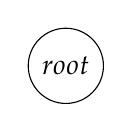
\begin{tikzpicture}[level/.style={sibling distance=60mm/#1}]
\node [circle,draw] (z){$root$}
;
\end{tikzpicture}}
\\
%%%% l = 2 
$\ell = 2 $ \ovalbox{
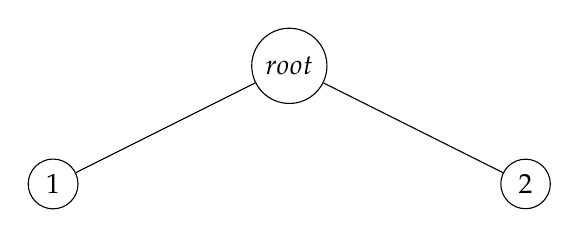
\begin{tikzpicture}[level/.style={sibling distance=60mm/#1}]
\node [circle,draw] (z){$root$}
  child {node [circle,draw] (a) {1} }
  child {node [circle,draw] (b) {2} }
;
\end{tikzpicture}}

%%%% l = 3
$\ell = 3 $ \ovalbox{
\begin{tikzpicture}[level/.style={sibling distance=60mm/#1}]
\node [circle,draw] (z){$root$}
  child {node [circle,draw] (a) {L}
  	child {node [circle,draw] (aa) {1}}
    child {node [circle,draw] (ab) {2}}
  }
  child {node [circle,draw] (b) {3} }
;
\end{tikzpicture}}

%%%% l = 4
$\ell = 4 $ \ovalbox{
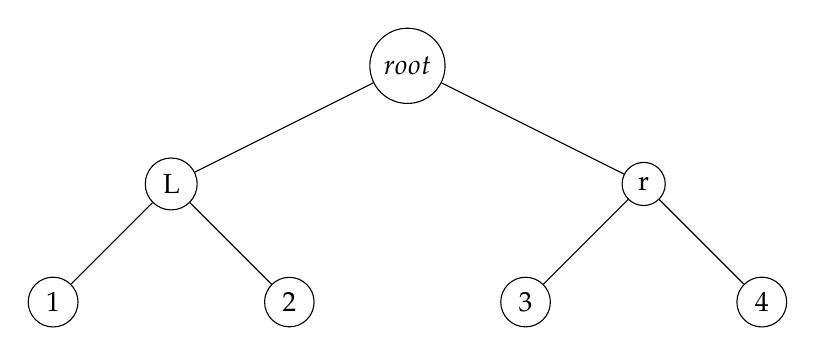
\begin{tikzpicture}[level/.style={sibling distance=60mm/#1}]
\node [circle,draw] (z){$root$}
  child {node [circle,draw] (a) {L}
  	child {node [circle,draw] (aa) {1}}
    child {node [circle,draw] (ab) {2}}
  }
  child {node [circle,draw] (b) {r} 
  	child {node [circle,draw] (ba) {3}}
    child {node [circle,draw] (bb) {4}}
    }
;
\end{tikzpicture}}

$\ell = 7 $ \ovalbox{
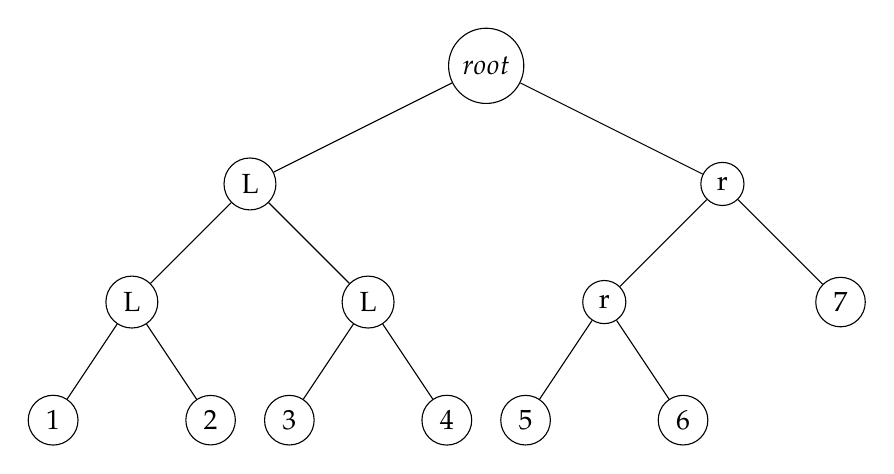
\begin{tikzpicture}[level/.style={sibling distance=60mm/#1}]
\node [circle,draw] (z){$root$}
  child {node [circle,draw] (a) {L}
  	child {node [circle,draw] (aa) {L}
    	child {node[circle,draw] (aaa) {1}}
		child {node[circle,draw] (aab) {2}}
        }
    child {node [circle,draw] (ab) {L}
   		child {node[circle,draw] (baa) {3}}
		child {node[circle,draw] (bab) {4}}
    }
  }
  child {node [circle,draw] (b) {r} 
  	child {node [circle,draw] (ba) {r}
    	child {node[circle,draw] (bbb) {5}}
        child {node[circle,draw] (bba) {6}}
    }
    child {node [circle,draw] (bb) {7}}
    }
;
\end{tikzpicture}}
\end{center}

We can see that an h-tree is an inherently recursive structure, 
which is either a full or complete binary tree. We cannot add leaf nodes to the
right subtree without filling up the leaft nodes on the left firstj

Base case: A single node is a full h-tree (base case of $\ell = 1 $) with 1
leaf node and an h-tree with an even number of nodes has a complete binary tree
as a left subtree. 

Inductive hypothesis: all h-trees are unique combinations of h-trees with lower
leaf node counts and the h-tree with $j<\ell$ nodes is an unique combination of
h-trees with nodes $<=j$. 

for $j = 3$, we can see that is the unique combination of the h-tree h-tree(1)
and h-tree(2) by the inductive step. Per definition, we can only add leaves on
from the left side of a tree and as $j=3 $ reduces to a combination of 1 and 3,
we can see that by the inductive hypothesis for all $j < \ell$ the pattern
holds.


Proof by induction:
\begin{proof}
For the height of the tree, we can see the base case of an h-tree is the
h-tree$(1)$ with height 0. For convienence sake, define $h(\ell)$ to be
the height of the h-tree with $\ell$ leaf nodes. We also know that a complete
binary tree has $2^h$ leaf nodes, so $\ell = 2^h$. 

Assume that when $\ell > 1$,  $ \exists j < \ell $ and that height of the h-tree is
indeed $lg(\ell)$\\
In our base case, we see $log(\ell) = log(1) = 0$ is true. \\
Inductive Hypothesis: \[ h(\ell) = log(\ell) \]

\begin{align*}
  h(\ell) &= h(2^h) \\
  log(\ell) &= log(2^h) \text{ (By IH)} \\ 
  log(\ell) &= h \\
\end{align*}
\end{proof}



\section{Parenthesization - again }
\begin{quote}
 \textbf{ Find the optimal Parenthesization for a matrix-chain product whose sequence
  of dimensions is: $(3,2,4,1,2)$. (Don't forget to include the table used to
computer your result.)}
\end{quote}

First diagonal:
\[ m_1 * m_2 = min \left( M(1,1) + m(2,2) + 24\right); k=1 \]
\[ m_2 * m_3 = min \left( m(2,2) + m(3,3) + 8 \right); k=2 \]
\[ m_3 * m_4 = min \left( m(3,3) + m(4,4) + 8 \right) k =3 \]


Second Diagonal:

\begin{align*}
	m_1 * m_2;\, (i = 2, j=4)\, min =  \begin{cases} 
				m(1,1) + m(2,3) + 6 \\
				m(1,2) + m(3,3) + 24 \\ 
			\end{cases} \\
	m_1 * m_4 , (i=1, j=4)\, min = \begin{cases}
				m(2,2) + m(3,4) + 2 \\
				m(2,3) + m(4,4) + 24 \\
			\end{cases} \\
	m_1 * m_4, (i =1, j=4 )\, min = \begin{cases}
				m(1,1) + m(2,4) + 12 \\
				m(1,2) + m(3,4) + 24 \\
				m(1,3) + m(4,4) + 6  \\
			\end{cases} \\
\end{align*}

tables:
\begin{table}[h]
	\caption{scalar values}
	\label{tab:mylabel}
	\begin{tabular}{|l|l|l|l|}
		\hline
		0 & 24 & 14 & 20 \\ \hline
		- & 0  & 8  & 24 \\ \hline
		- & -  & 0  & 8  \\ \hline
		- & -  & -  & 0  \\ \hline
	\end{tabular}
\end{table}

\begin{table}[h]
	\caption{k values}
	\label{tab:kval}
	\begin{tabular}{|l|l|l|l|}
		\hline
		0 & 1 & 1 & 3 \\ \hline
		- & 0  & 2  & 3 \\ \hline
		- & -  & 0  & 3  \\ \hline
		- & -  & -  & 0  \\ \hline
	\end{tabular}
\end{table}

final parentization:
\[ \left( (m_1 (m_2 m_3)) m_4 \right)\]

\section{Donut buying problem}
\begin{quote}
	\textbf{A bakery sells donuts in boxes of three different quantities, $x_1, x_2,
		x_3$. In the Donut Buying problem, you are given the numbers $x_1, x_2,
		x_3$, and an integer $n$ and you should return either }
	\begin{enumerate}
		\item \textbf{the minimum number of boxes needed to obtain exactly $n$ donuts if
			this is possible, along with a set of boxes that obtains this minimum}
		\item \textbf{``DOH'' if it is not possible to obtain exactly $n$ donuts. }
	\end{enumerate}
	\textbf{For example, if $x+1 = 4, x_2 =6, x_3 = 9, \text{and } n=17$, then you should
	return that 3 boxes suffices, with 2 boxes of size 4, and 1 box of size 9.
	However, if n=11, you should return DOH! since it is not possible to buy
exactly 11 donuts with these box sizes. }
\end{quote}

\subsection{For any positive $x$, let $m(x)$ be the minimum number of boxes
  needed to buy $x$ donuts if this is possible, or INFINITY $\infty$
  otherwise. Write a recurrence relation for the value of $m(x)$. Don't forget
the base case(s)!}

\subsubsection{answer}
We havea base case of $n=0$, in which the solution is also 0. We also must have
as a precondition that at least one of $x_1 \lor x_2 \lor x_3 \leq n $ or we have
no solution. Given

\begin{align*}
	m(x) = \begin{cases}
		0 \text{ if } n = 0 \\
		min_{i:x_i \leq n} \left(1 + m(n - x_i)\right) \\
	\end{cases}
\end{align*}



\subsection{ Give an efficient algorithm for solving Donut Buying. How does its
  running time dpeend on $x_1, x_2, x_3,\text{ and } n$? Is it an algorithm
that runs in polynomial time in the input sizes?} 

\subsubsection{answer}
In pseudocode, we can implement the algorithm. 

\begin{lstlisting}
def findBoxes(b[ ], n) :
	boxFinder[0] = 0 
	boxes[]
	minBoxes = ``doh''
	for i in range(1:n):
		if b[i] <= n:
			if 1 + boxFinder[n - b[i]] < minBoxes:
				boxFinder = [ 1 + boxFinder[n - b[i]
				boxes[i] = b[i]

	if boxFinder.isEmpty() == true: 
		return minBoxes

\end{lstlisting}
The algorithm has one for loop that iterates the list of boxes and does several
comparisons along the way $O(cn + \Theta(1)$ = $0(n)$ and uses $O(n)$ extra
space. 



\section{Viterbi Algorthm}
	\subsection{find the sequence}
\begin{quote}
	\textbf{Note in this problem, a label can appear on more than one edge in the graph
		and can even appear on more than one edge leaving a given node in the graph.
		\\
		We can use dynamic programming on a directed graph $G = (V,E)$ for speech
		recognition. Each edge $(u,v) \subset E$ is labeled with a sound
		$\sigma(u,v)$ from a finite set $\Sigma$ of sounds. The labeldd graph is a
		formal model of a person speaking a restricted language. Each path in the graph
		starting from a distinguised vertex $v_0 \subset V$ corresponds to a possible
		sequence of sounds produced by the model. We define the label of a directed
		path to be the concatenation of the labels of the edges on that path. 
		Describe an efficient algorithm that, given an edge-labeld graph
		$G$ with distinguised vertex $v_0$ and a sequence $s = \langle \sigma_1,
		\sigma_2, \dots, \sigma_k \rangle$ of sounds from $\Sigma$, returns a path in
		$G$ that begins at $v_0$ and has $s$ as its label, if any such path exists.
		Otherwise, the algorithm should return \textsc{no-such-path}. Analyze the
		running time of your algorithm. (Hint: you may find conceps from Chapter 22
	useful.)}
\end{quote}

\subsubsection{Answer}
We have to first find the distinguised vertex. Assuming we've found that
vertex, we can start a breadth-first search from there to find a path with the
correct sequence. Assuming our graph $G$ is stored in an adjacency list and our
distinguised vertex is $v$

Note that we do not need to store the examined edges in a table - we can simply
use a queue-backed variant of breadth-first search to search for a path, and
given that we have a smaller subproblem of finding just the sequence $\sigma_1,
\sigma_2$, (or formally, $\sigma_k, \sigma_{k+1}, k<n$. If we find that, we can add the edges containing it to a list with
the edge indices. As we continue searching the graph, if the sequence
$\sigma_i, \dots \sigma_n$ is found, we can return that specified path and if
it isn't found when the graph search is exhausted, we return
\textsc{no-such-path}. 
Since our graph is stored in an adjacency list and we must potentially traverse
all the edges of the graph, we have an expected running time of $O(V+E) +
\Theta(1)= O(V+E) $ and we use $O(cE) = O(E) $ extra space.
  	
\subsection{adding probabilities}

\begin{quote}
	\textbf{Now, suppose that every edge $(u,v) \subset E$ has an associated
		nonnegative probabilty $(p(u,v)$ of traversing the edge $(u,v)$ from
		vertex $u$ and thus producing the corresponding sound. The sum of the
		probabilities of the edges leaving any vertex equals 1. The probabilty of
		a path is defined to be the product of the probabilities of its edges. We
		can view the problem of a path beginning at $v_0$ as the probabilty that a
		``random walk'' beginning at $v_0$  will follow the specified path, where
		we randomly choose which edge to take leaving a vertex  $u$ according to
		the probabilities of the available edges leaving $u$. 
		Extend your answer to part (a) so that if a path is returned,
		it is a most probable path starting at $v_0$ and having label s. Analyze
	the running time of your algorithm. }
\end{quote}

\subsubsection{Answer}
Given that more than one sequence of sounds can be found, (more than one edge
leaving a node can be labeled the same) we can adapt our list to a small table
that contains the potential path edges from a given vertex as they are found.
This makes the solution to this part easier, as we can calculate the
probabilities of each path as well and return the path with the greatest
probability. In practice, this would likely be accomplised by adding
probability information to an edge object to make calculating the max probable
path simple.



\section{The Chicken Brothers} 
\begin{quote}
Gus wants to open franchises of his restuarant, Los Pollos Hermanos,
along Central Avenue. There are $n$ possible locations for franchises where
location $i$ is at mile $i$ on Central. Each location $i>1$, is thus a distance
of 1 mile from the previous one. There are two rules.
\begin{itemize}
\item At each location there can be at most one restaurant, and the profit of a
  restaurant at location $i$ is $p_i$. 
  \item Any two restaurants must be at least 2 miles apart.
\end{itemize}
\end{quote}
\subsection{ Jesse proposed the following algorithm: Sort the locations by
  decreasing $p_i$ values, then greedily choose the next possible location,
  provided that it doesn't conflict with previously choses locations. Show that
Jesse's algorithm doesn't always give maximum profit.}

\subsubsection{answer}
Is we have the set of profits at locations $P = \{5, 8, 9, 10, 9\}$ and sorted
them to get $\{10, 9, 9, 8, 5\}$, Jesse's algorithm would choose the store with
profit 10 and 8 (the two stores with profits 9 are too close to the store with
profit 10. The optimal answer in this example is selecting the 1st, 3rd, and
5th locations. ($23 > 18$). 

\subsection{Now consider a dynamic programming approach to this problem. For
  $i\geq 0 \text{let } m(i)$ be the maximum profit obtainable by using
  locations 1 throught $i$. Write a recurrence relation for $m(i)$. Don't
forget the base case(s).}
We have two base cases:
$ m(1) = p_1 , m(2) = max(p_1, p_2)$. 

\begin{align*}
m(i) = max \begin{cases} 
		  m(i-1)  \\
		  m(i-2) + p_i\\
\end{cases}
\end{align*}

\subsection{Describe how you would create a dynamic program using the previous
recurrence. What is the run time of your algorithm?} 

We can see the following dynamic program for this problem:
\begin{lstlisting}
def findMaxProfit(int[] profit):
  int[] maxProfit
  maxProfit[0] = profit[0]
  if profit.length == 1:
	return maxProfit[0]

  for x in range(0, len(profit):
	if x == 1:
	  maxProfit[x] = profit[x]
	maxProfit[x] = max(profit[x-1], profit[x-2] + profit[x])
  return maxProfit[profit.length-1]
\end{lstlisting}

At most, this algorithm iterates over the profit array once, with constant
runtime for the assignment and reads, giving a runtime of $\Theta(n)$.

\subsection{now Gus wants to solve a generalization of the problem. There are
  two changes. First, for $1 < i \leq n$, location $i$, is now distance $d_i$
  from location $i-1$. Second, any two restaurants must now be distance $k$
  appart for some parameter $k$. Write a new recurrence relation for this
problem. Don't forget the base case(s).}

$ m(1) = p_1 , d_i - k > i\,,, m(2) = max(p_1, p_2)$. 

\begin{align*}
	m(i) = max_{d_i -k > i} \begin{cases} 
		  m(i-distance(i, i-1))  \\
		  m(i-k) + p_i\\
\end{cases}
\end{align*}


\end{document}
